\documentclass[12pt]{article}
\usepackage{gensymb}
\usepackage{graphics}
\usepackage{graphicx}
\graphicspath{{storage/self/primary/Download/asgnt8/fig}}
\graphicspath{{storage/self/primary/Download/asgnt8/table}}
\usepackage{amsmath}
\usepackage{float}
\let\vec\mathbf
\usepackage{float}
\providecommand{\brak}[1]{\ensuremath{\left(#1\right)}}
\providecommand{\myvec}[1]{\ensuremath{\begin{pmatrix}#1\end{pmatrix}}}
\providecommand{\norm}[1]{\ensuremath{\lvert|#1\rvert|}}
\begin{document}
\title{\textbf{11.11.1.13}}
\date{}
\maketitle
\textbf{Question :} Find the equation of the circle with radius 5 whose centre lies on $x$-axis and passes through the point $\brak{2,3}$.

\textbf{Solution :}
\begin{table}[H]
    \centering
       \begin{tabular}{|c|c|c|}
    \hline
    \textbf{Input Parameters} &\textbf{Description} &\textbf{Value} \\
    \hline
     $\vec{O}$& Center(at origin)&$\vec{0}$\\
     \hline
 $r$ & Radius &1\\
 \hline
 $\theta$&-&$100\degree$\\
 \hline
 $\alpha$&-&$165.4\degree$\\
 \hline
 $\beta$&-&$5\degree$\\
 \hline
  \end{tabular}

    \caption{Table of input parameters}
    \label{tab:11.11.1.13}
\end{table}
The general formula of the circle is
\begin{align}
\norm{\vec{x}}^2 + 2\vec{u}^{\top}\vec{x}+f&=0\\
 where,   \vec{u}=-\myvec{6\\0}\\
 \norm{\vec{A}}^2 + 2\vec{u}^{\top}\vec{A}+f&=0\\
 or,f&=11
\end{align}
Therefore the equation of the circle is
\begin{align}
   \norm{\vec{x}}^2 - 2\myvec{6&0}\vec{x}+11&=0
\end{align}    
\begin{figure}[H]
    \centering
	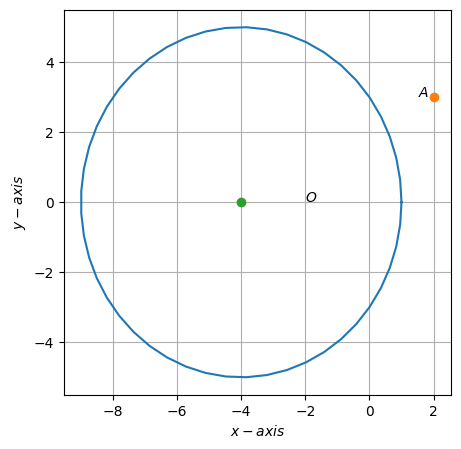
\includegraphics[width=\columnwidth]{fig/11.11.1.13.png}
    \caption{}
    \label{fig:11.11.1.13}
\end{figure}
\end{document}

